\section{失效分析}

\subsection{轴承结构建模分析}
轴承结构建模是一个系统性的过程,用于描述和分析轴承的工作原理、性能和可能的问题。其包括:
(1) 基本几何建模:
基本几何建模包括考虑包括内圈、外圈、滚动体(如球或滚柱)、保持架和密封件的几何尺寸、形状和布局。
(2) 材料与物性分析:
该部分考虑轴承材料,如轴承钢、陶瓷等,以及它们的机械和热学性质(如硬度、弹性模量、热膨胀系数等)。
(3) 动力学建模:
该部分考虑轴承在运行时的动态行为,如旋转、振动和受力情况。使用多自由度系统动力学方程来描述轴承的动态行为。
(4) 摩擦和磨损分析:
该部分需要分析轴承中的摩擦现象,考虑摩擦力、热产生和可能的磨损模式。了解摩擦和磨损对轴承性能和寿命的影响。

在轴承研究的解析模型部分,动力学模型的构建是一个核心焦点。目前,轴承动力学模型涵盖了多种类型,如静力学模型、动力学模型、非线性模型以及有限元模型。具体来说,静力学模型主要关注轴承的受力分析,而不涉及其运动状态;有限元模型则针对轴承结构进行深入分析和设计;动力学模型考虑到轴承的实际运动,帮助研究其在不同操作条件下的振动行为和动态反应;而非线性模型则更适用于在高速和大负荷等特殊条件下探究轴承的非线性属性。

在本报告中,我们专注于对轴承的动态特性进行建模。初步阐述了轴承的内部工作机制,并基于轴承的运动状态、表面波纹度、接触刚度和Hertz接触力等要素,制定了二阶动力学方程。进一步地,我们深入研究了在故障情境下的动态方程。特别关注了由于局部缺陷导致的球与内外滚道之间的位移变动,揭示了这种位移如何引发振动响应的过程。这些分析为轴承故障检测提供了坚实的理论基础和数据支撑。

\subsubsection{正常模型的分析}
尽管滚动轴承的几何设计非常精确,但在运行时仍然会出现振动现象。这主要归因于滚动体与内、外圈之间的有限滚动接触,这些接触点具有其固有的弹性特性。为了深入理解轴承的动态行为,我们可以建立一个专注于其正常运行时的动力学模型。这种动力学模型在考虑到一些假设和简化前提后,通常分为单自由度和多自由度的系统模型。

1、单自由度系统模型

在单自由度系统模型中,我们将轴承系统简化为一个独立的质点的动态模型。这种简化模型假设在水平方向上,轴承系统可以被视为一个单一质点的运动,并且这个质点会受到外部载荷的影响。其具体的运动模式如下:
\begin{equation}
    m\ddot{x}+c\dot{x}+kx=F(t),
\end{equation}
其中,$m$是质点的质量;$x$是质点的位移;$\dot{x}$和$\ddot{x}$分别是质点的速度和加速度;$c$是阻尼系数;$k$是刚度系数;$F(t)$是外部载荷。


这种模型常被称为“二阶动力学模型”,因其基于二阶微分方程描述。为了确定这个模型的参数,我们可以利用实验技术和数学分析工具进行识别。

2、多自由度系统模型

多自由度系统模型描述了轴承系统不能被简化为单一质点运动的情况。相反,它包含多个相互作用的组件和多个质点。相对于单自由度系统模型而言,多自由度系统模型更为复杂。

通过使用拉格朗日方程,我们可以建立多自由度系统模型,并通过求解该模型得到系统的自然频率、阻尼和刚度等参数。多自由度系统模型的主要优势在于它能够考虑轴承系统中多个部件之间的相互作用,从而更准确地描述轴承的动力学行为。
\begin{figure}[!ht]
  \centering
  \includegraphics[width=0.6\linewidth]{figures/C3/fig3 modelZN.eps}
  \caption{轴承简化结构模型}
  \label{fig:轴承简化结构模型}
\end{figure}



轴承正常动力学模型的构建可以采用单自由度系统模型或多自由度系统模型。这些模型能够更全面地反映轴承系统的动力学特性。

滚动轴承的动力学模型直接由滚动体与滑道之间的接触特性决定。尽管滚动轴承的组件相对简单,但其内部运动和变形接触却十分复杂,尤其在制造工艺误差的影响下,波纹度会影响各组件之间的相对运动。当轴承发生故障时,其运动模型也将相应改变。因此,本部分研究了由加工误差引起的波纹度和缺陷对球和滚道之间接触特性的影响,以推导轴承的动力学方程。轴承的主要构件包括外圈、内圈、球和保持架,它们的简化结构模型可以分别描述其功能和相互作用。


\subsubsection{波纹度影响}

滚动轴承的振动主要与其波纹度有关。在轴承工作时,位于内外圈之间的滚动体(在此指为球体)会产生圆周式的移动。然而,由于制造过程的限制,内外圈和滚动体的表面并不是完全平滑的。因此,真正的圆周移动只会在完全光滑的轨道上实现,而在现实中考虑到波纹度时,球与轨道的接触会导致接触角的变化以及接触面曲率半径的变更,从而影响接触应力的分布。图~\ref{fig:波纹度模型}展示了轴承部件外表面的整体正弦形状的波纹度模型,其中波纹度的特征波长远远大于球与导向环之间赫兹接触面积的尺寸。我们用波数表示每周长波的数量。波纹度缺陷的存在揭示了球在轨道上运动的实际轨迹,明显表明其不是严格意义上的圆周运动,而是伴随着曲率变化的运动。



波纹度会使轴承在运行时的接触载荷发生变化。这种变化的程度与波纹度的深度和接触点的刚度密切相关。由于这种接触载荷的波动,轴承会出现振动。以下是外圈与第$j$个球接触点的波纹度数值:
\begin{equation}
\label{eq2:波纹度1}
    P_{oj} = p_{m}\sin{[N_{o}(\omega_{c}t+\frac{2\pi(j-1)}{Z})+\eta_{o}]},
\end{equation}
式中$\omega_{c}$为保持架(Cage)的旋转角速度,$p_m$为外圈波纹度最大幅值,$N_o$是外圈的$N$个波纹,$Z$表示球的个数,$\eta_{o}$则是外圈波纹度的初始相位角。
同理内圈与第$j$个球接触处的波纹度值是:
\begin{equation}
\label{eq2:波纹度2}
P_{i j}=A_i \sin \left[N_i\left(\left(\omega_c-\omega t\right) t+\frac{2 \pi(j-1)}{Z}\right)+\beta_0\right],
\end{equation}
式中$A_i$表示内圈波纹度的最大幅值,$\omega_c$ 是保持架旋转速度,$\omega$ 是主轴旋转速度,$\beta_0$是内圈波纹度的初始相位角,$q_m$是内圈波纹度最大幅值。那么对于球而言,它同时和内圈和外圈接触,并且两者在相位上相差$\pi$,因此球在接触点处的波纹度值为:
\begin{equation}
\label{eq2:波纹度3}
    u_{b j}=A_{m}\left[\sin \left(N_{b} \omega_{b}+\gamma_{0}\right)+\sin \left(N_{b}\left(\omega_{b}+\pi\right)+\gamma_{0}\right)\right],
\end{equation}
其中 $\omega_b$是球自转速度, $\gamma_0$为球波纹度值得初始相位角, $A_m$是球波纹度最大值。
\begin{figure}
  \centering
  \includegraphics[width=0.55\linewidth]{figures/C3/fig2.jpg}
  \caption{波纹度模型}
  \label{fig:波纹度模型}
\end{figure}


%%%%%%%%%%%%%%%%%%%%%%%%%%%%%
%%%%% 这一个part可以删除 %%%%%%
%%%%%%%%%%%%%%%%%%%%%%%%%%%%%
% \subsubsection{接触刚度}
% 接触刚度受接触面曲率和接触材料的影响。用下标 $\romannumeral1$表示球,$\romannumeral2$表示滚道。通过球和滚道接触面的法线,与轴承径向平面夹角为 $\alpha$的平面被称作第1平面,通过球心的轴向平面为第2平面。因此,可以分别表示球与外圈接触副的主曲率、球和内圈接触副的主曲率、球和外圈接触副的曲率以及球-内圈的曲率。

% 接触刚度$K$是由接触面的曲率和接触材料共同决定的。在此,下标 $\romannumeral
% 1$代表球,而 $\romannumeral2$ 代表滚道。接触面的法线与轴承的径向平面构成了一个角度$\alpha$ 这被称为第1平面。与此相对,通过球心的轴向平面定义为第2平面。因此,我们可以分别描述球与外圈接触的主曲率、球与内圈接触的主曲率,球与外圈的副曲率,以及球与内圈的副曲率。
% 	\begin{equation}
% 	\label{sec1:subsec1:eq1}
% 	\rho_{\uppercase\expandafter{\romannumeral1}-1} = \rho_{\uppercase\expandafter{\romannumeral1}-2} =\frac{2}{D_b},	\rho_{\uppercase\expandafter{\romannumeral2}-1} =-\frac{2}{D_o},\rho_{\uppercase\expandafter{\romannumeral2}-2} =-\frac{1}{r_o},
% 	\end{equation}
% 式子中:$D_b$表示球的直径,$D_o$和$D_i$分别表示外圈滚道直径和内圈滚道的直径。$r_o$和$r_i$分别表示外圈曲率半径和内圈曲率半径。

% % \begin{equation}
% % 	\label{sec1:subsec1:eq2}
% % 	\rho_{\uppercase\expandafter{\romannumeral1}-1} = \rho_{\uppercase\expandafter{\romannumeral1}-2} =\frac{2}{D_b},   	\rho_{\uppercase\expandafter{\romannumeral2}-1} =\frac{2}{D_i},\rho_{\uppercase\expandafter{\romannumeral2}-2} =-\frac{1}{r_i}
% % 	\end{equation}

% 接着可以表示出球轴承的主曲率$\sum {\rho}$和其主曲率函数$F(\rho)$,下式分别给出了球和内圈、球与外圈以及轴承的主曲率和主曲率函数表达式:


% 接着,我们可以描述球轴承的主曲率为 
% $\sum {\rho}$,并定义其主曲率函数为 
% $F(\rho)$。以下公式展示了球与内圈、球与外圈以及整体轴承的主曲率和相应的主曲率函数表达式:
% \begin{equation}
%  \label{sec1:subsec1:eq2}
% 	\begin{split}
% 	    	\sum {\rho_{\uppercase\expandafter{\romannumeral1}} } &= \rho_{\uppercase\expandafter{\romannumeral1-1}} + \rho_{\uppercase\expandafter{\romannumeral1-2}} = \frac{4}{D_b} ,\\
% 	    	\sum {\rho_{\uppercase\expandafter{\romannumeral2}} } &= \rho_{\uppercase\expandafter{\romannumeral2-1}} + \rho_{\uppercase\expandafter{\romannumeral2-2}} = -(\frac{2}{D_o} + \frac{1}{r_o} ),\\
% 	    	\sum {\rho } &= \rho_{\uppercase\expandafter{\romannumeral1}} + \rho_{\uppercase\expandafter{\romannumeral2}}.
% 	\end{split}
% \end{equation}
    
% 此刻,球与内圈或外圈滚道之间的载荷-变形关系,也就是接触刚度 $K^{\prime}$,可以通过椭圆积分和椭圆率的适当表达式进行计算:






%     \begin{equation}
%     \label{sec1:subsec1:eq5}
%         K'=\left(\frac{\pi^{2} k^{2} E^{\prime 2} K(e)}{4.5 L^{3}(e) \sum \rho}\right)^{0.5}
%     \end{equation}
%     利用~\eqref{sec1:subsec1:eq1}-\eqref{sec1:subsec1:eq5}分别求出$K_i$ 和$K_o$。其中$E’$为等效弹性模量,其可以用下列式子表示出:
% \begin{equation}
% \frac{1}{E^{\prime}}=\frac{1}{2}\left(\frac{1-v_a^2}{E_a}+\frac{1-v_b^2}{E_b}\right),
% \end{equation}
% 式子中,$E$表示选用的弹性模量,$v$表示泊松比,下标表示所选取物体,这里$a$和$b$分别表示物体$a$和$b$。另外:
% \begin{equation}
% \begin{aligned}
%     k &= \frac{b}{a},\\
%     K(e) &= 1.5277 +0.6023 \ln{(\frac{\sum \rho_1}{\sum \rho_2})},\\
%     L(e) &= 1.0003 +0.5968(\frac{\sum \rho_1}{\sum \rho_2}),\\
%     K &=1.0339(\frac{\sum \rho_1}{\sum \rho_2})^{0.636},
% \end{aligned}
% \end{equation}
% 其中,$a$表示椭圆接触面的长半轴,$b$为接触椭圆面的短半轴,$k$表示短半轴与长半轴之比,$K(e)$和$L(e)$分别为椭圆参数,代表了第一类和第二类全椭圆积分。
    
% 最终表示出刚度系数$K_j$
%     \begin{equation}
%         K_j = [\frac{1}{(\frac{1}{k_i})^{q} + (\frac{1}{k_o})^{q} }]^{q},
%     \end{equation}
% 其中,$q$表示载荷-变形指数,当轴承的滚动体为球时,$q=3/2$;当滚动体是圆柱滚子时,$q=10/9$。





\subsubsection{Hertz接触力}

国内外的研究表明,轴承动力学的理论领域内,Hertz的接触振动理论(1881年)揭示了球与轴承之间座圈的非线性接触特性。尽管该理论并未全面描述滚动轴承的所有运动特性,但它的基本前提是严格的,并为我们提供了简化的力学公式,其计算误差通常较小。因此,Hertz接触理论在轴承动力学模型的构建中仍是主要的参考方法。在这个理论框架下,滚动轴承的接触力是沿着特定的接触角产生的。这个接触角的正负性取决于接触体(无论是内圈还是外圈)的曲率中心位置。如果曲率为正,那么接触角也是正;反之,则为负。

此外,Hertz接触理论的核心假设是接触体之间仅有弹性形变力,并遵循胡克定律。这一理念被用来描述滚珠与轴承的接触振动,将滚珠在轴承内部视为一个质量为零的“非线性接触弹簧”,并将这弹簧的两端分别与内外圈相连接,如图~\ref{fig:Hertz模型}所示。运动时每个球在滚道上$x-y$平面的实时位置如下所示:
\begin{equation}
\phi_j=\omega_c t+\frac{2 \pi(j-1)}{Z},
\end{equation}
其中,$Z$是轴承滚道上的球总数, 是第 个球的实时位置(弧度)。其分布如~\ref{fig:轴承简化结构模型}所示。
\begin{figure}
  \centering
  \includegraphics[width=0.9\linewidth]{figures/Chap02fig/fig4.pdf}
  \caption{轴承非线性Hertz模型}
  \label{fig:Hertz模型}
\end{figure}
其中$K_j$是由内圈和外圈的刚度系数确定的接触刚度。为了简化模型,将接触刚度$K_j$设置为只与材料相关的时不变值[37]。

刚度系数可以通过上一节的式~\eqref{sec1:subsec1:eq5}表示.这里$K_i$和$K_o$分别是内外圈和球之间的接触刚度系数。此外,刚度系数实际上与接触材料的泊松比和接触曲率有关。 另一个参数$\delta_j$是球和座圈之间的弹性变形。弹性形变是外圈发生振动前后内外圈沟道中心距离的差值,首先需要定义出未发生振动的初始差值:
刚度系数可以由上述式子 ~\eqref{sec1:subsec1:eq5}来表示。在这里,
$K_i$和$K_o$ 分别代表内圈与外圈、以及球体之间的接触刚度。值得注意的是,刚度系数与接触材料的泊松比和接触曲率密切相关。另外,参数 $\delta_j$ 描述了球体与座圈之间的弹性形变,它表示了在外圈振动前后,轴承内外圈中心间的距离变化。为了清晰起见,我们首先需要确定在振动发生前的初始距离差值。

\begin{equation}
B_d=r_{g i}+r_{g o}-D_b+G_r,
\end{equation}
其中 $r_{gi}$是内圈沟道的中心;$r_{go}$是外圈沟道的中心;$D_{b}$是球的直径,$G_{r}$是径向游隙。对于同一个轴承,以上参数均视为常数。接着便表示出外圈发生振动后的内外圈沟道中心差值:
\begin{equation}
B_d^{\prime}=\sqrt{\left(x \cdot \cos \left(\phi_j\right)+y \cdot \sin \left(\phi_j\right)+B_d \cdot \cos \left(\alpha_0\right)\right)^2},
\end{equation}
在不考虑油膜影响的情况下,无负载下的内圈和外圈中心之间的差值$B_d$和负载状态下内圈和外圈的差值$B_{d}^{'}$外圈振动之前的差值,即第$j$个球的弹性变形为:
\begin{equation}
\delta_j=B_d^{\prime}-B_d-u_{b j}-\gamma,
\end{equation}
式子中$\gamma$表示径向游隙。

根据Hertz接触理论,第$j$个球与滚道者之间的接触力$F_j$表示为:
\begin{equation}
\label{eq:elastic deformation}
F_j=K_j \delta_j^{1.5},
\end{equation}

球轴承中的球的反作用力在$y$方向将会被表示为:
\begin{equation}
\begin{aligned}
& F_{j y}=K  \delta_j^{1.5}  \sin \phi_j.\\
\end{aligned}
\end{equation}

\subsubsection{正常轴承动力学模型}
尽管五自由度的轴承模型提供了更为详尽和全方位的信息,以真实反映轴承的运动轨迹,但本研究重点关注轴承在
$y$轴方向的加速度。因此,简化的二自由度模型已足够为我们提供
$y$轴方向的动力学方程。

在实践中,对轴承的状态进行持续监测显得尤为重要。在工业应用中,为了了解轴承的状态,通常会检测其振动信号。实际上,我们测量到的球轴承振动信号主要源于外圈的振动。这意味着作用于外圈的弹簧力是由滚珠与外圈之间的Hertz接触力所决定的总和。
\begin{equation}
\begin{aligned}
& F_x=\sum_{j=1}^Z F_{y j}. \\
\end{aligned}
\end{equation}

此时,滚动轴承二自由度的非线性系统动力学可以用牛顿第二定律表示:
\begin{equation}
\begin{aligned}
& m \ddot{y}+c_y \dot{x}+F_y=m g,\\
\end{aligned}
\end{equation}
式子中,$m$表示轴承的质量,$\ddot{x}$和$\ddot{y}$分别是轴承在$X-Y$坐标系中的位移加速度。

\subsection{轴承故障失效分析}

\subsubsection{理论分析}
轴承的故障主要可归结为两大类:分布式故障与局部缺陷。在实际的工业应用中,大约有90\%的故障都是由局部缺陷造成的。因此,本研究重点深入探讨了局部缺陷对轴承性能的影响。当轴承滚道出现局部缺陷时,这将导致轴承的动力学模型发生改变,尤其是外圈所受的Hertz接触力将有明显的变动。

凹痕通常是因为碎片、压痕或表面的磨损所引起的,这些凹痕的大小通常远小于轴承各个组件的尺寸。值得注意的是,这些凹痕并不是使球掉入其中,而是会在球上滚动。

在国际研究中,对于故障轴承的局部缺陷建模,有学者采用基于冲击力的方法,通过模拟周期性的冲击来描述轴承故障对动力学方程的效应。虽然这种方法在仿真中相对简便,但与实际情况有所偏差。同时,其他研究者采纳近似的策略,将缺陷描述为规则的几何形状,并考虑其对弹性变形的瞬时影响,进而影响球的受力情况,从而对轴承的动力学方程产生影响。因此,本研究假设滚动轴承滚道上的局部故障为一个简化的矩形凹痕。如图~\ref{fig:外圈局部缺陷}所示。

\begin{figure}
  \centering
  \subcaptionbox{外圈上的局部缺陷\label{fig:外圈局部缺陷}}
    {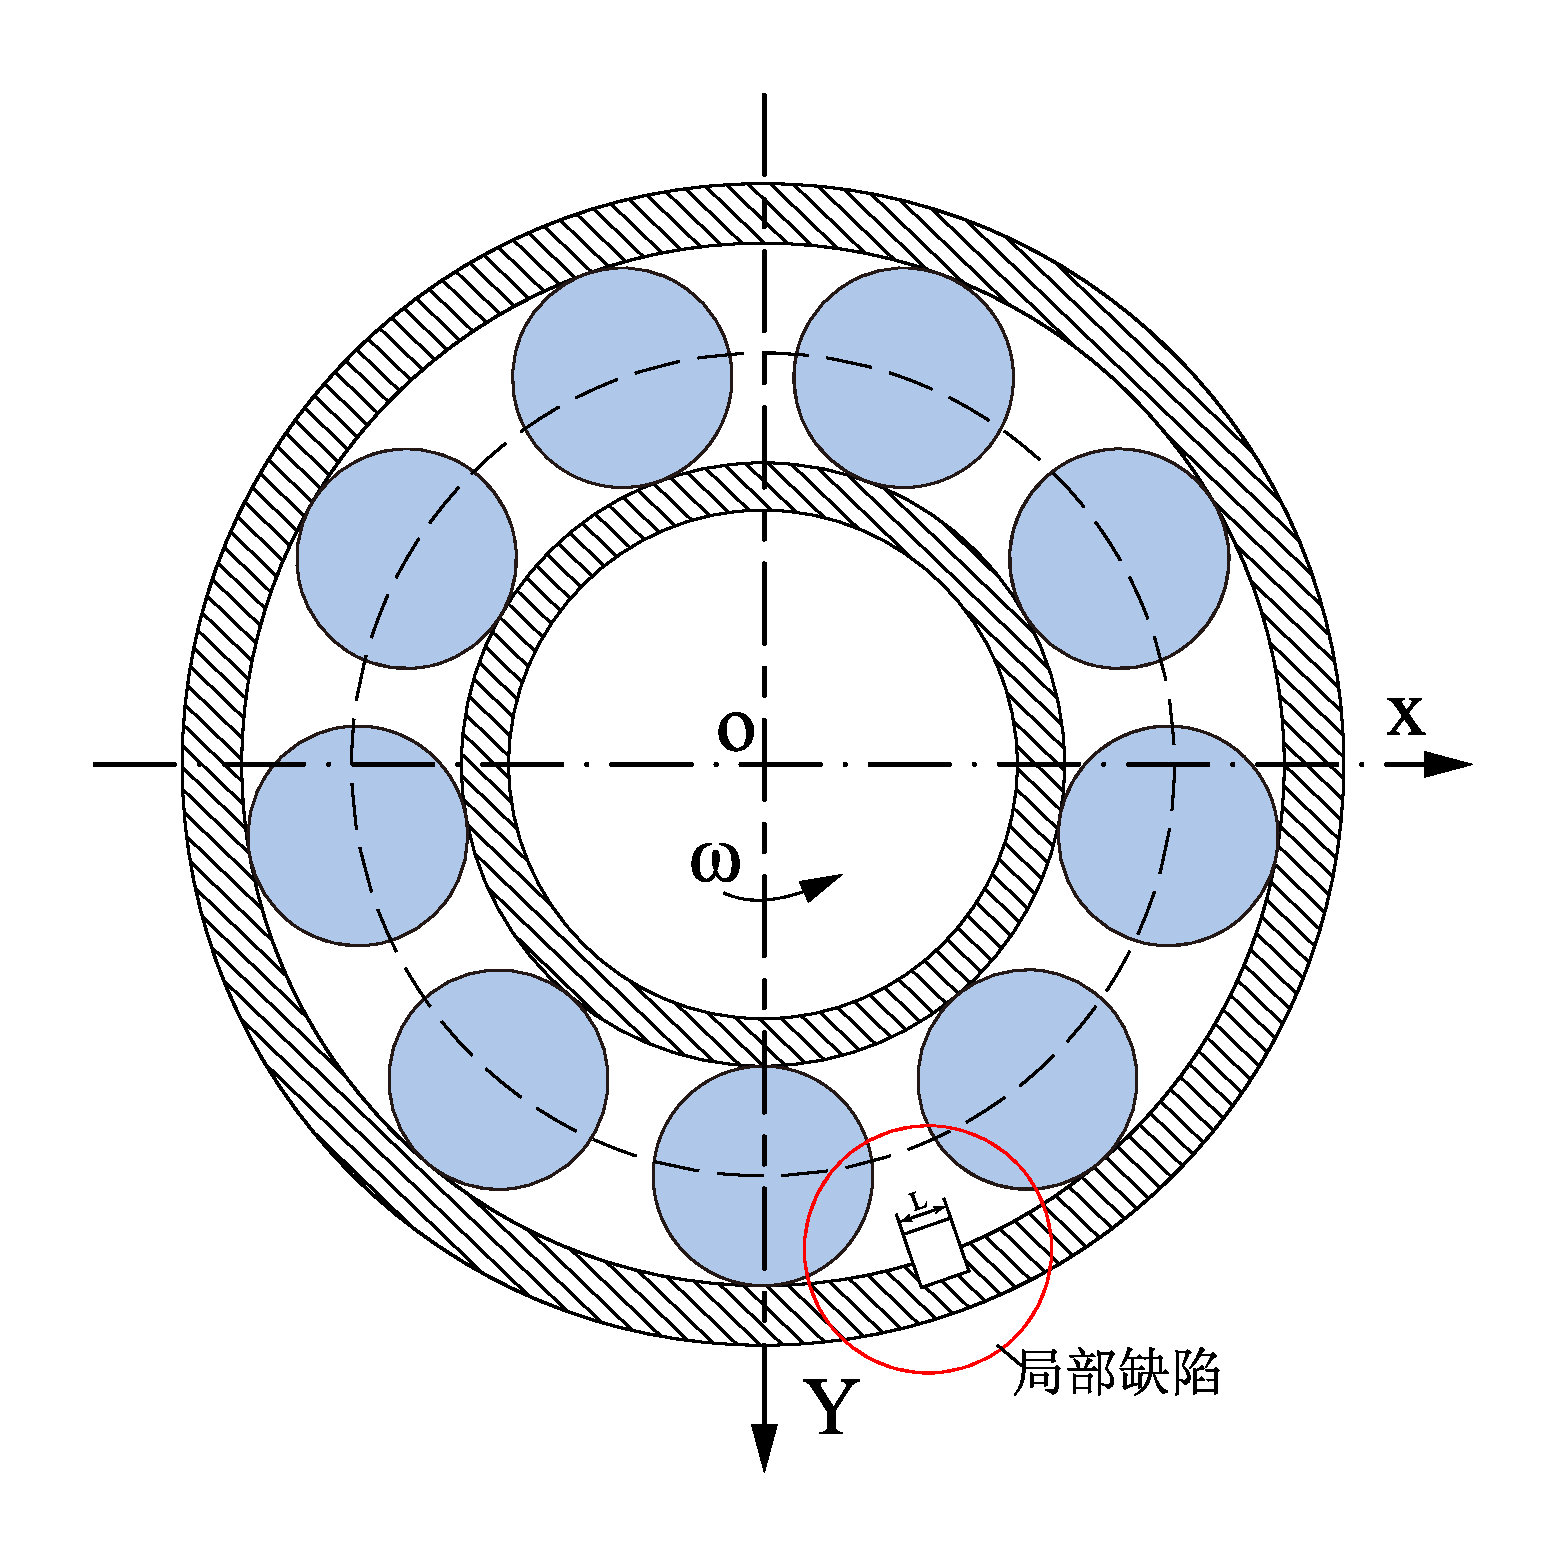
\includegraphics[width=0.45\linewidth]{figures/C3/fig6.pdf}}
  \subcaptionbox{局部几何缺陷俯视图和侧视图\label{fig:subfig-b}}
    {\includegraphics[width=0.45\linewidth]{figures/C3/fig5-1.pdf}}
%  \caption{局部缺陷}
\end{figure}

% \begin{figure}
%   \centering
%   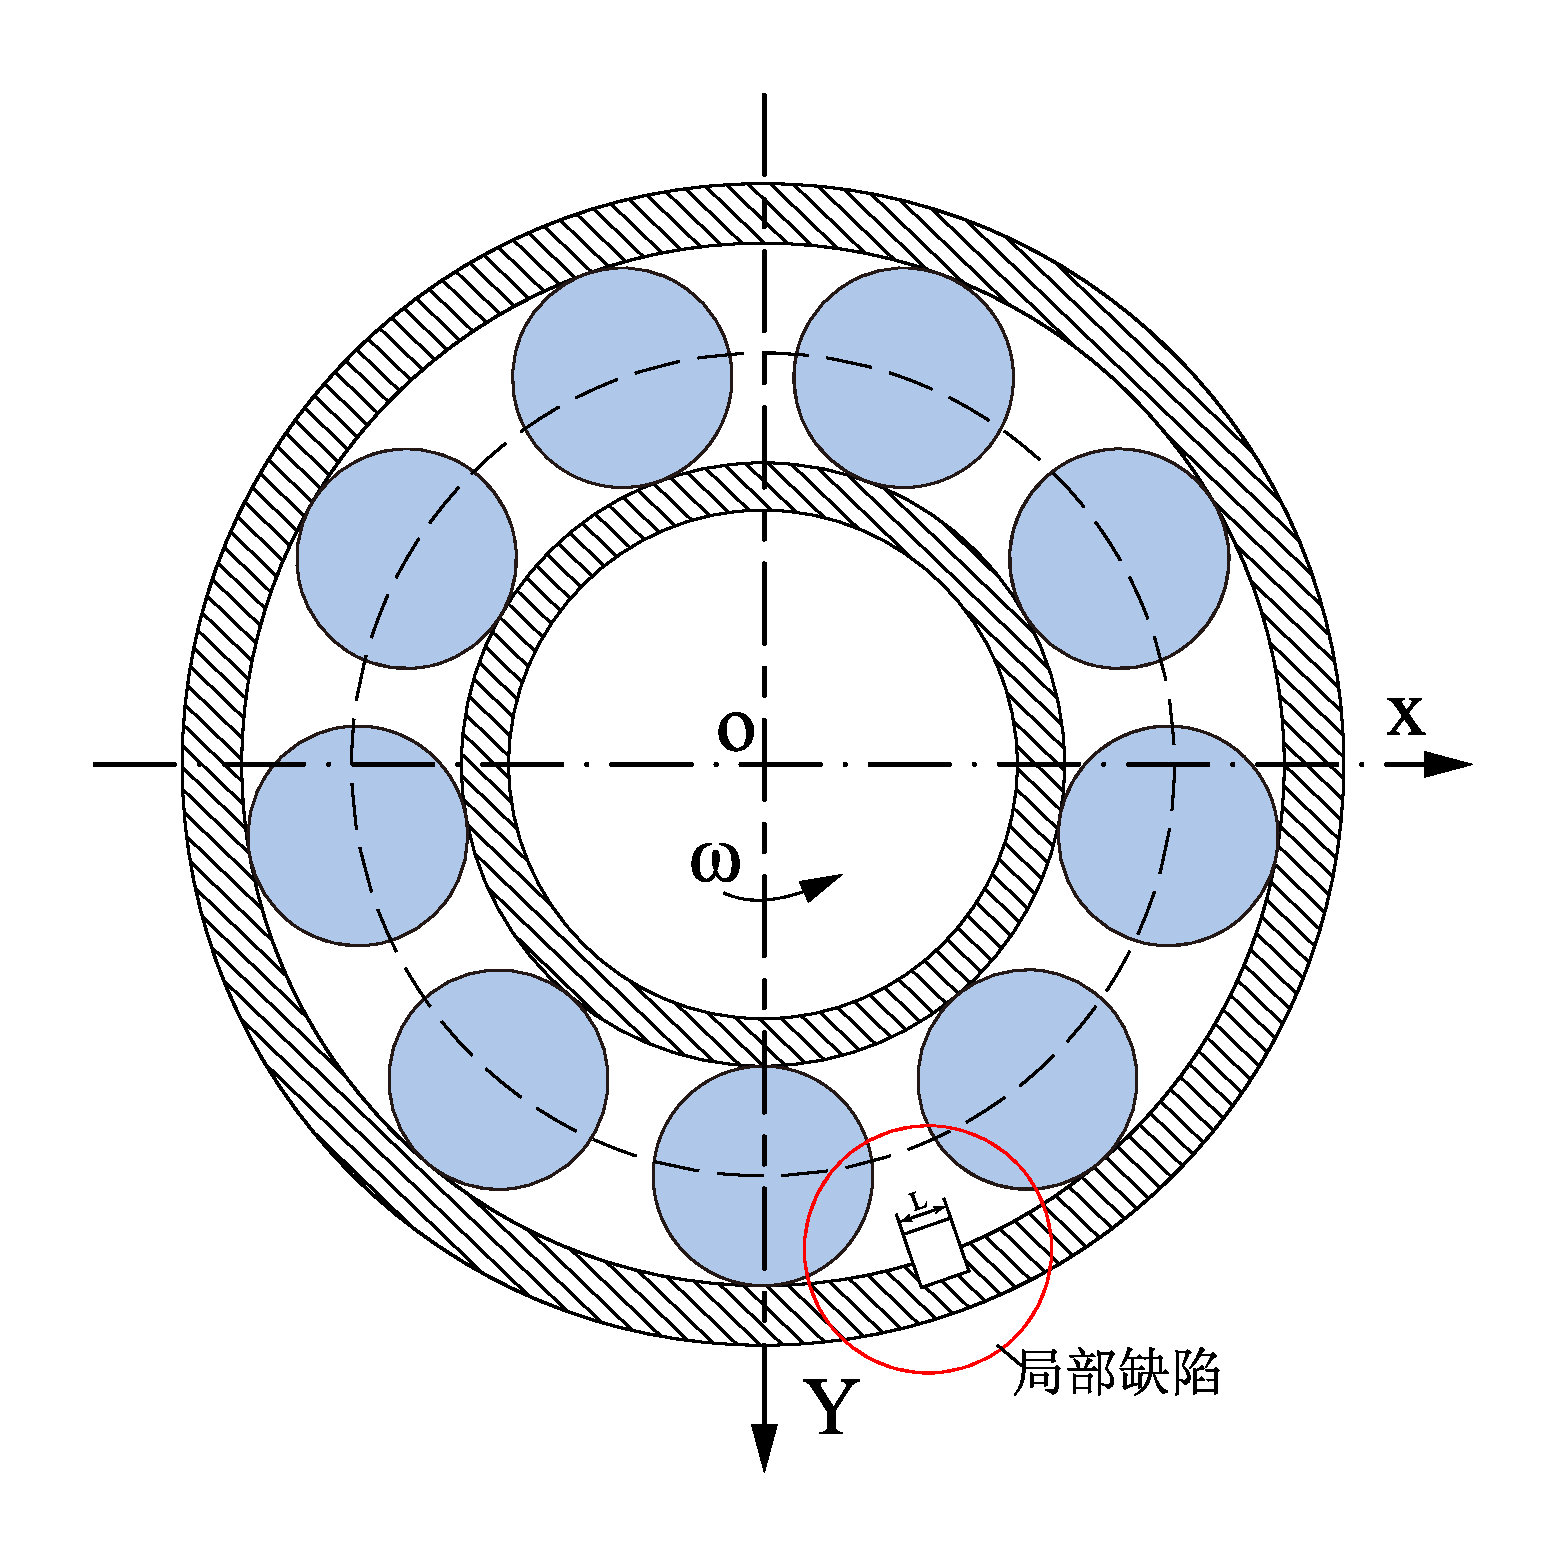
\includegraphics[width=0.5\linewidth]{figures/C3/fig6.pdf}
%   \caption{外圈上的局部缺陷}
%   \label{fig:外圈局部缺陷}
% \end{figure}

% 当滚动轴承滚道表面存在局部缺陷时,以外圈局部故障为例,首先使用直径$L$和深度$H$定义凹痕的物理性质,其故障位置的几何关系如图~\ref{fig:故障俯视图和侧视图}所示。
% \begin{figure}
%   \centering
%   \includegraphics[width=0.6\linewidth]{figures/Chap02fig/fig5.png}
%   \caption{局部几何缺陷俯视图和侧视图}
%   \label{fig:故障俯视图和侧视图}
% \end{figure}

球在正常滚道上运动时,其弹性形变$\delta_j$将不会发生变化,只有当其运动到缺陷位置时,弹性形变$\delta_j$会由于接触变化而产生变化,从而影响了轴承的运动。在上一节中已经阐明,根据Hertz接触理论,球与内外圈之间属于点接触,其载荷-弹性形变关系式如下式所示:

当球在正常的滚道上滚动时,其弹性形变
$\delta_j$ 是恒定的,不会有变化。但是,当球滚动至某个有缺陷的位置时,接触情况发生变化,导致弹性形变
$\delta_j$ 随之改变,进而影响了轴承的整体运动。正如前文所述,基于Hertz接触理论,球与内、外圈的接触是点对点的,其载荷与弹性形变之间的关系可以表示为以下公式:
\begin{equation}
F_j=K_j \delta_j^{n},
\end{equation}

其中,$n$代表载荷-变形指数,这一指数与缺陷的大小直接相关。过去的研究者提出,对于球形结构,它的载荷-变形指数的工程近似为$n=1.5$。故其Hertz接触力的计算仍如式~\eqref{eq:elastic deformation}所示。


在本文中,我们采用了分段函数来描述球经过缺陷时的运动行为和建模策略。鉴于早期的缺陷往往相对较小,因此我们没有详细探讨大型缺陷所引入的复杂分段函数模型。我们专注于考虑球的尺寸大于缺陷的尺寸,且这个缺陷是一个长方形,其长度明显大于其宽度的情况。如图~\ref{fig:球与局部缺陷接触关系示意图}所示。
\begin{figure}
  \centering
      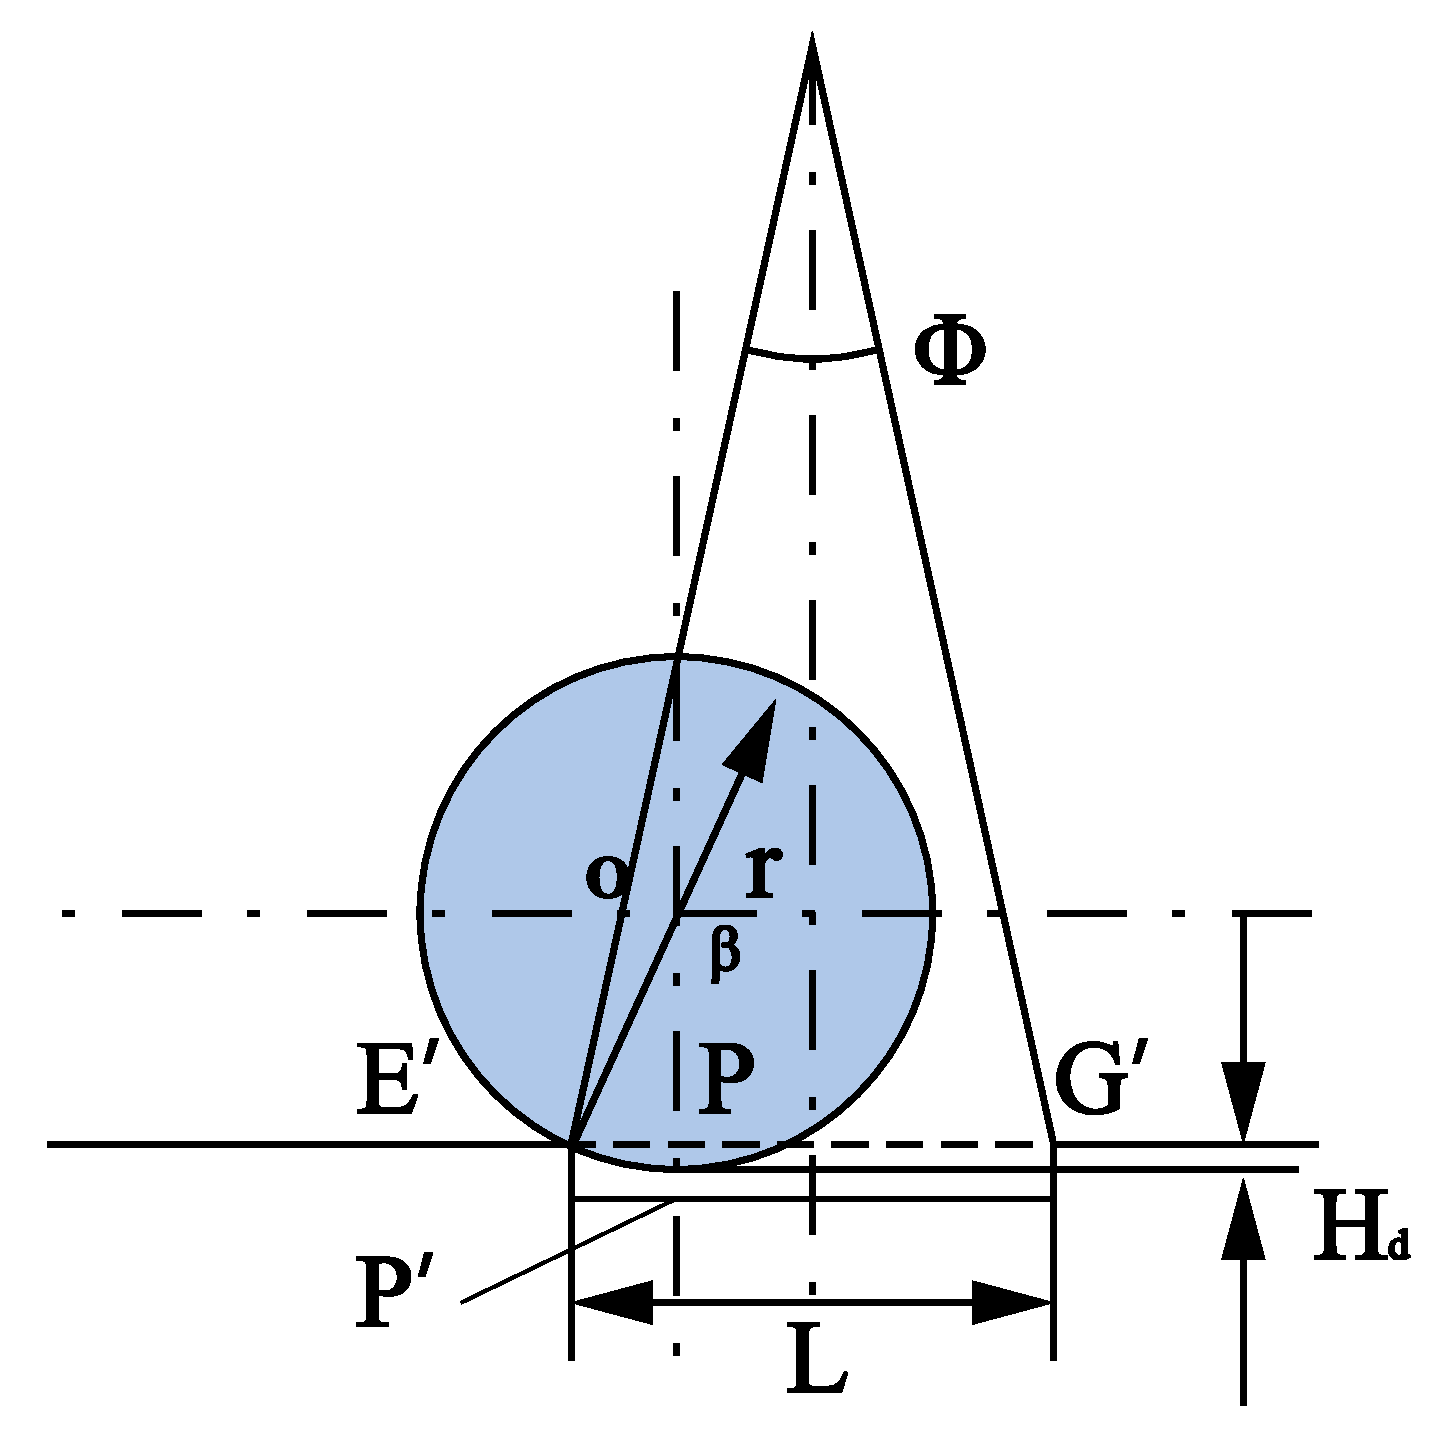
\includegraphics[width=0.3\textwidth]{figures/C3/fig8.pdf}
  \caption{球与局部缺陷接触关系示意图}
  \label{fig:球与局部缺陷接触关系示意图}
\end{figure}

当球经过故障区域时的接触行为可以描述为以下几个步骤:首先,球开始与缺陷的起始边产生接触,并随后与其两侧边产生总计三个接触点;接着,球从缺陷的起始边脱离,仍然与其侧边保持接触,但尚未接触到缺陷的终止边,此时只有两个接触点;最后,当球即将到达缺陷的结束边时,其接触状态与进入缺陷时的状态相似,又重新形成三个接触点。随后,球将返回到正常的滚道上,恢复其正常的滚动状态。具体的接触过程如图~\ref{fig:接触过程示意图}所示。
\begin{figure}[h]
  \centering
  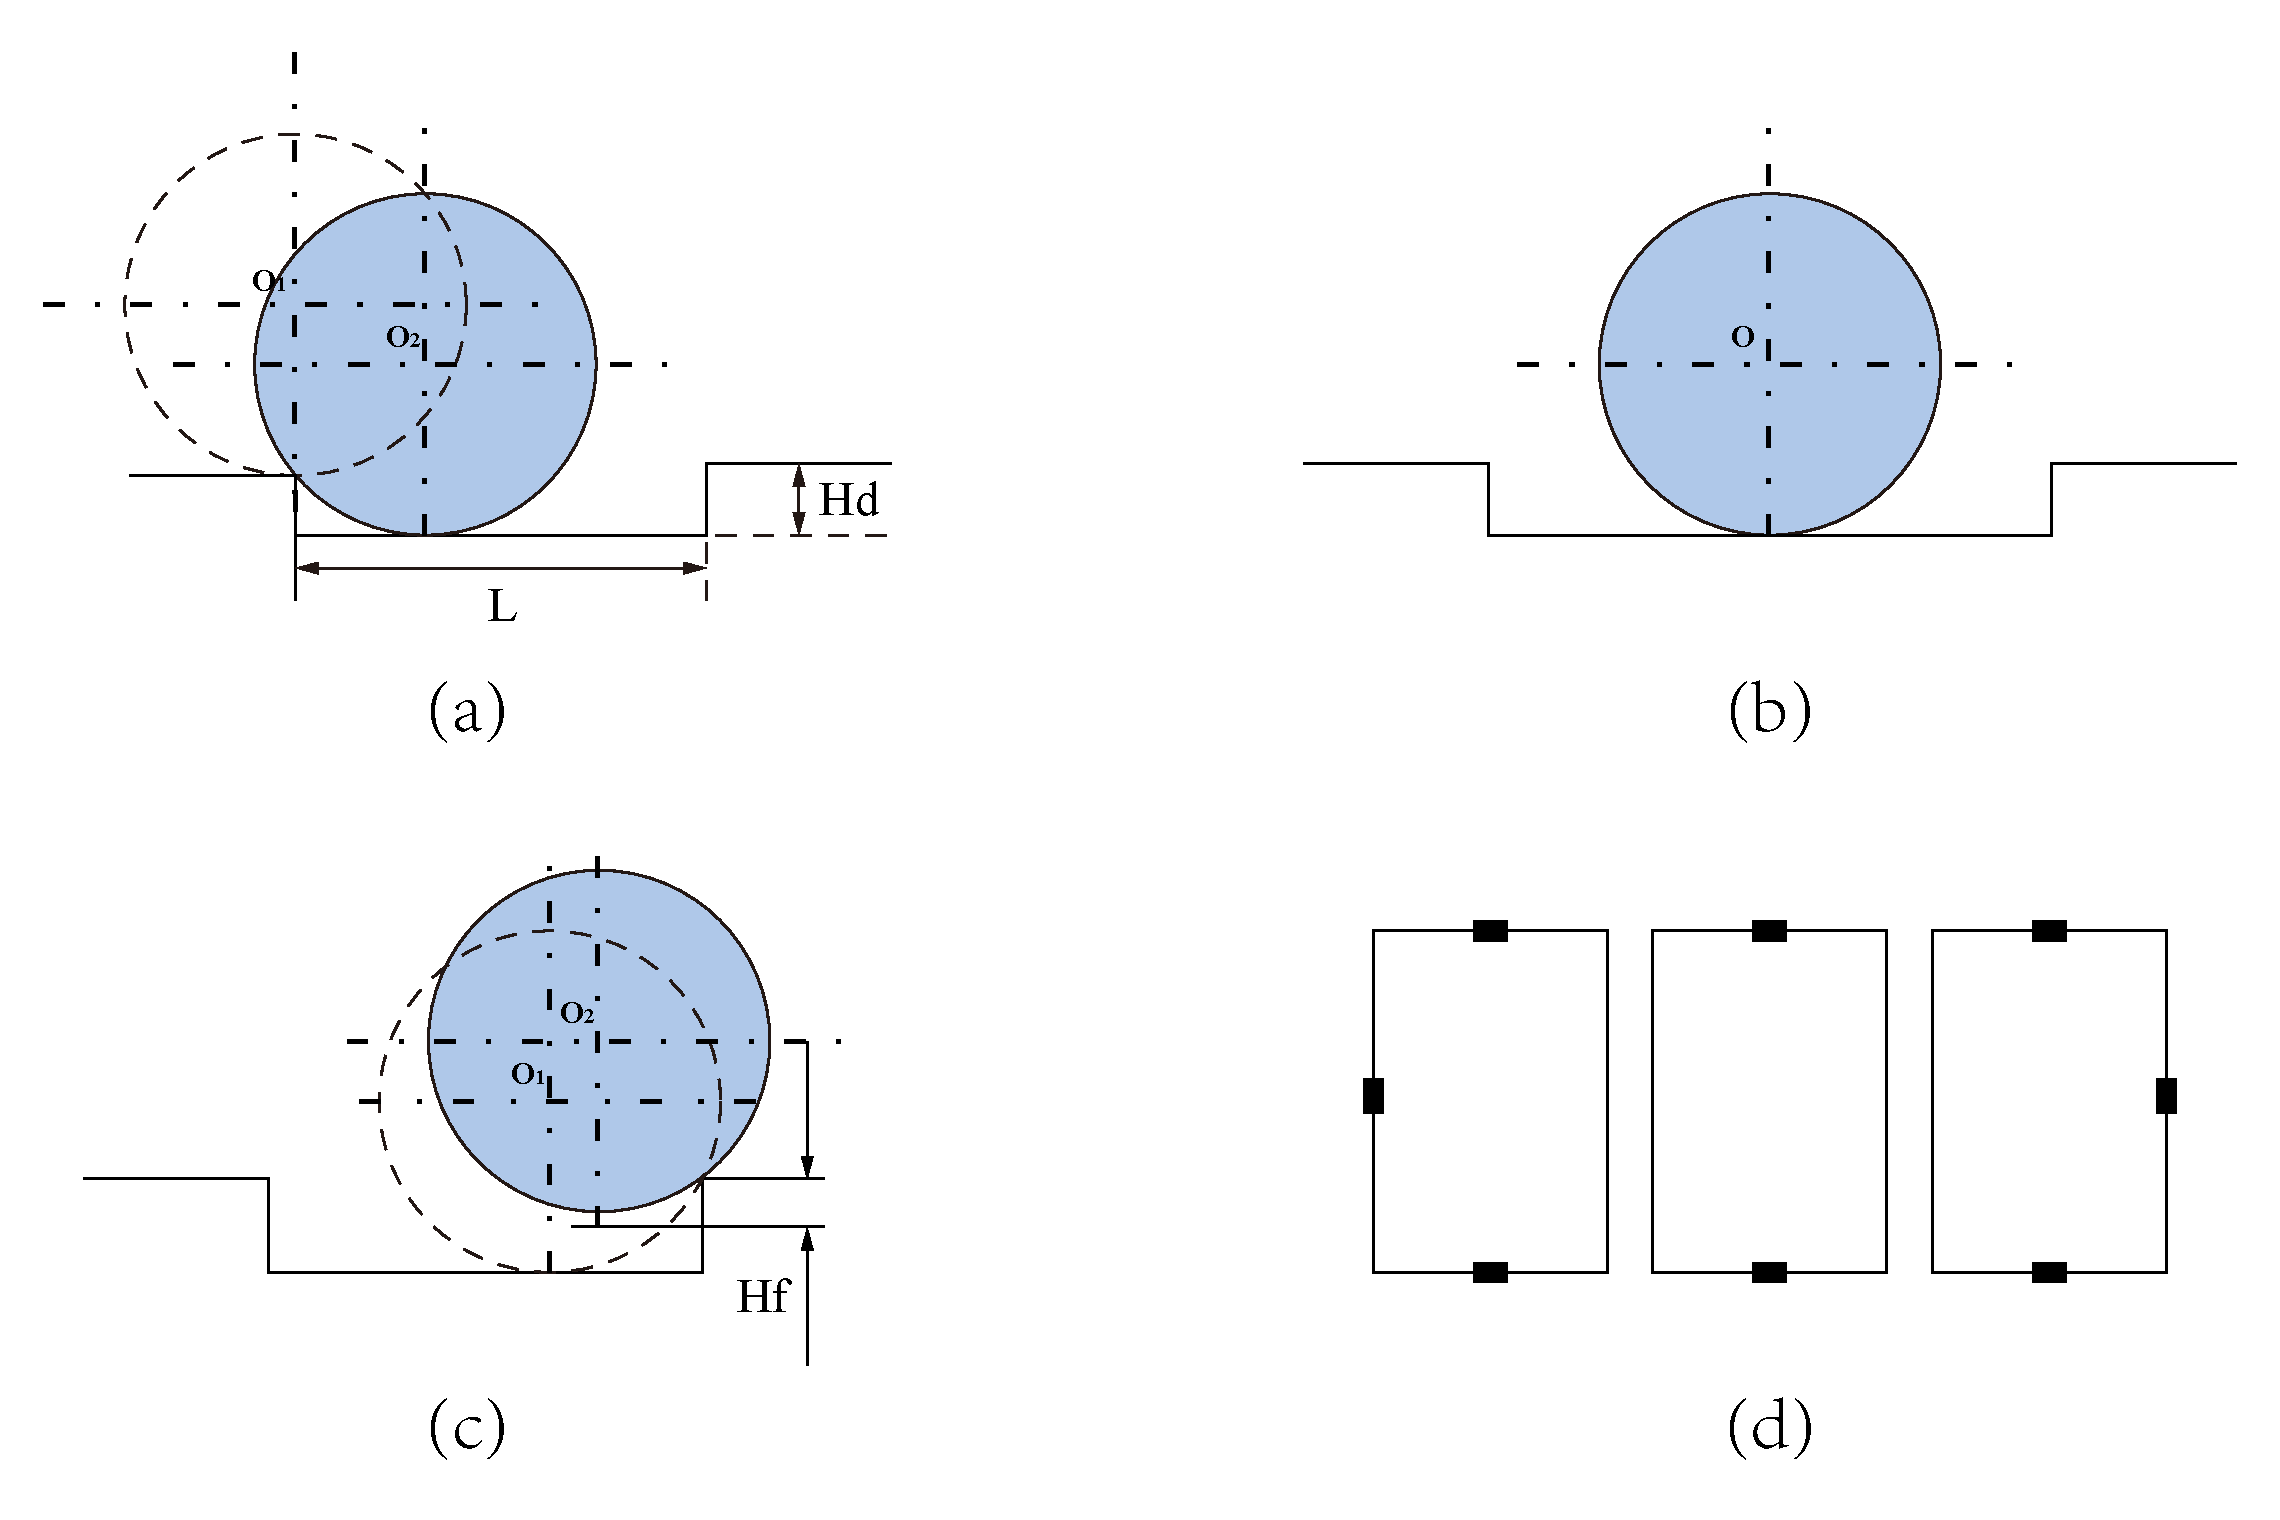
\includegraphics[width=0.7\linewidth]{figures/C3/fig9.pdf}
  \caption{接触过程示意图}
  \label{fig:接触过程示意图}
\end{figure}

基于以上的分析可构造出分段函数模型,如图~\ref{fig:分段函数}所示。
\begin{figure}
  \centering
  \includegraphics[width=0.6\linewidth]{figures/C3/fig7partfunction.png}
  \caption{分段函数示意图}
  \label{fig:分段函数}
\end{figure}

定义轴承中第$j$球的实时角度为:
\begin{equation}
\phi_{r j}=\bmod \left(\phi_j, 2 \pi\right),
\end{equation}
式子中$\bmod(.)$表示为取余函数。

弹性形变$\delta_j$的变化主要是来源于球与局部缺陷的接触的消失及恢复,当引入故障后,其新的位移可以具体地表达出来:
\begin{equation}
H_{f j}=\left\{\begin{array}{lc}
H_d \sin \left(\frac{\pi \cdot \phi_{r j}-\phi_0}{2 \Delta T}\right) & \phi_0 \leq \phi_{r j} \leq \phi_0+\phi_f \\
0 & \text { otherwise }
\end{array}\right.,
\end{equation}
其中,$\phi_0$是缺陷的初始角度,$\phi_f$是缺陷占据的角度,$\Delta T$是缺陷占据的时间。$H_d$是球进入缺陷区域后接触变形的变化量,即滚道与球圆心距的变化量。其最大值是缺陷的深度$H$,但是一般而言故障早期的缺陷深度$H$远小于球的直径,因此$H_d$可以由下式计算得出:
\begin{equation}
H_d=0.5 d-\left[(0.5 d)^2-(0.5 W)^2\right]^{0.5}.
\end{equation}

另外由于缺陷可能出现在外滚道或内滚道,其表达式可以用下式表示为:
\begin{equation}
\Delta T=\left\{\begin{array}{l}
\arcsin \left(\frac{L}{D_0}\right) \\
\arcsin \left(\frac{L}{D_i}\right)
\end{array}\right.,
\end{equation}
因此最终的有缺陷的弹性变形$\delta_j$表示为:
\begin{equation}
\delta_j^{\prime}=\delta_j-H_{f j},
\end{equation}
则局部缺陷球轴承在$y$方向的总接触力分别表示为: 
\begin{equation}
\begin{aligned}
F_y^{\prime}=\sum_{j=1}^z K \varsigma_j \delta_{e j}^{1.5} \sin \phi_j,
\end{aligned}
\end{equation}
其中,$\varsigma_j$为第$j$个球的载荷区系数,其表达式为:
\begin{equation}
\zeta_j= \begin{cases}1 & \delta_j>0 \\ 0 & \delta_j \leq 0\end{cases},
\end{equation}
$\delta_{e j}$为第 $j$个球的总接触变形,其表示为:
\begin{equation}
\delta_{e j}=x \cos \theta_j+y \sin \theta_j-\gamma-u_{b j}-H_{f j}.
\end{equation}

基于二自由度正常球轴承动力学模型,同时考虑本节的局部缺陷引入的时变位移激励模型,则局部缺陷球轴承的二自由度动力学方程表示为:
\begin{equation}
\label{eq2:dynamics}
\begin{aligned}
m \ddot{y}+c \dot{y}+\sum_{j=1}^Z K_e \varsigma_j\left(x \cos \theta_j+y \sin \theta_j-\gamma-H^{\prime}\right)^{1.5} \sin \theta_j=mg.
\end{aligned}
\end{equation}
\subsubsection{仿真实验}


为了验证轴承动力学模型的可靠性和实用性,我们在python中,根据建模结果进行仿真实验,观察一定负载下,健康轴承和故障轴承加速到某固定速度后匀速运动时y方向的加速度。

\begin{table}[htbp]
    \centering
    \begin{tabular}{|c|c|}
    \hline
        参数名 & 参数值 \\\hline
         滚珠数量&8\\\hline
         轴承负载&1kg\\\hline
         转速&600rpm\\\hline
         仿真步长&$2\times10^{-5}s$ \\\hline
         故障深度&$3\times 10^{-6}$ \\\hline
         材料刚度&$3.2\times 10^7$  \\\hline
         径向游径&$5\times10^{-6}$\\\hline
         
         随机噪声&$10^{-5}\times G(0,0.1)$\\\hline
    \end{tabular}
    \caption{部份仿真参数}
    \label{tab:sim_label}
\end{table}

仿真中,我们在轴承$\frac\pi3$处外侧滑道上人为设定一个半宽度为$\frac\pi{20}$。轴承总负载为1kg,重力加速度为$g=9.8$m/s$^2$。解算方法为欧拉法。部份参数如表\ref{tab:sim_label}。

根据该模型,当轴承处于完全健康状
态时,轴承时域图和频谱图中理论上不会出现冲击成分,轴承的运转基本处于平
稳状态。下图展现了健康轴承与故障轴承在负载为1kg情况下,短时间内加速到600rpm后的y方向加速度的观测。可以观察到,健康轴承运转过程中,除加速过程中的正常加速度外,在稳定运行时几乎没有出现抖动,没有出现较大的冲击成分。而故障轴承在运行过程中,出现了明显的具有周期运动规律的抖动,如图\ref{fig:sim_time_0.05, fig:sim_time}所示。

对这两种情况进行快速傅立叶变换,获得两种轴承运行过程中的频谱图。可以观察到,在特定的频率上,故障轴承的频谱具有明显较高的幅度,如图\ref{fig:sim_freq}所示。

最后,将我们的仿真结果与 [15] 中针对相同故障类型轴承在定速工况下的仿真结果进行了对比。对于故障轴承,其仿真响应如图 \ref{fig:sim_benchmark} 所示。可以观察到,两者在时域冲击特征及频域包络谱结构上具有较高的一致性,这也在一定程度上验证了我们所建立的模型及分析方法的合理性与正确性。

% \begin{figure}
%   \centering
%       \includegraphics[width=0.65\textwidth]{figures/C3/10.png}
%   \caption{正常轴承动力学模型求解图}
%   \label{fig:正常轴承动力学模型求解图}
% \end{figure}

\begin{figure}[htbp]
  \centering
      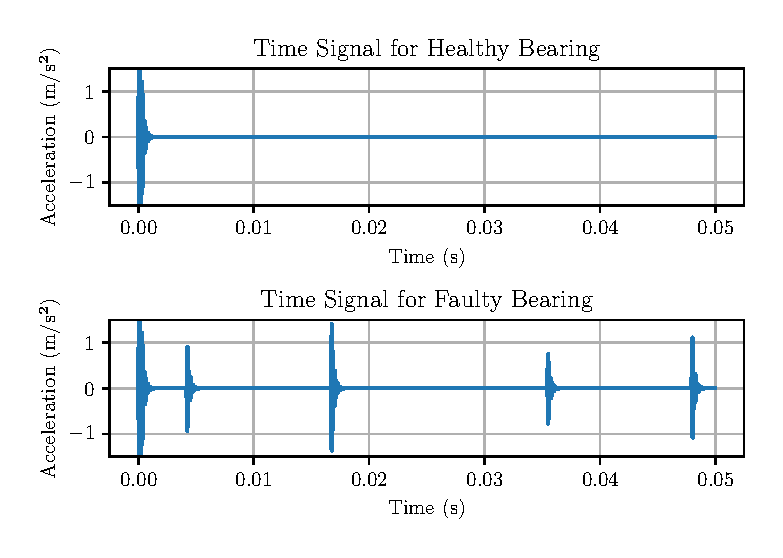
\includegraphics[width=0.65\textwidth]{figures/C3/sim/time_signals_0.05.eps}
  \caption{仿真结果的时域图(前0.05秒)。上图为健康轴承,可以观测到其仅在加速阶段在y方向有明显的加速度;下图为故障轴承,在某些时刻会出现冲击信号。}
  \label{fig:sim_time_0.05}
\end{figure}

\begin{figure}[htbp]
  \centering
      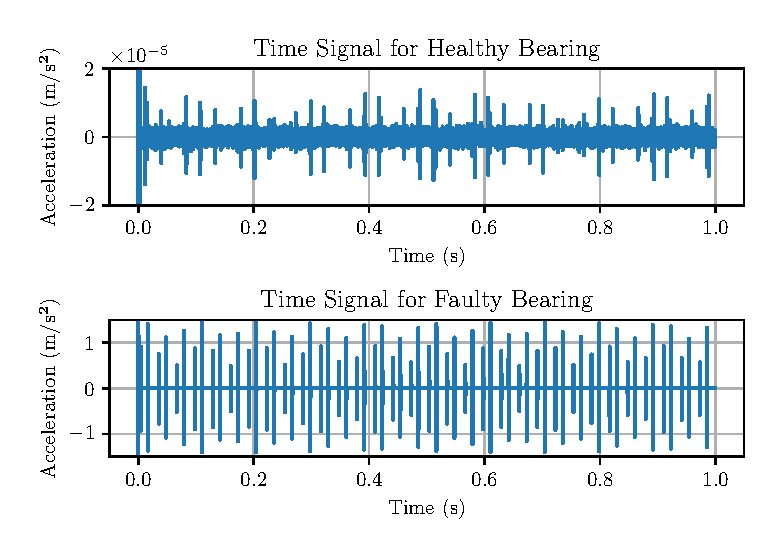
\includegraphics[width=0.65\textwidth]{figures/C3/sim/time_signals.eps}
  \caption{仿真结果的时域图(前1秒)。可以观察到健康轴承(y坐标轴缩放到$10^{-5}$数量级)在除加速阶段外,y方向加速度仅存在波纹或噪声。}
  \label{fig:sim_time}
\end{figure}

\begin{figure}[htbp]
  \centering  \includegraphics[width=0.65\textwidth]{figures/C3/sim/fft_compare.eps}
  \caption{经过快速傅立叶变换(FFT)的健康轴承和故障轴承y方向时域信号100Hz~150Hz的表现。可以观察到,在特定频段(如127Hz处),故障轴承的频谱强度明显高于健康轴承。}
  \label{fig:sim_freq}
\end{figure}

\begin{figure}[htbp]
  \centering
    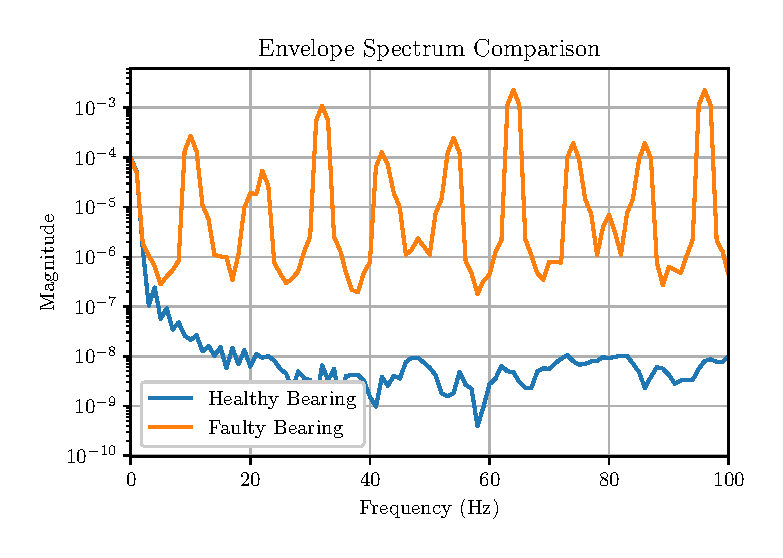
\includegraphics[width=0.65\textwidth]{figures/C3/sim/envelope_spectrum_comparison.eps}
  \caption{对加速度信号进行带通滤波。健康轴承的包络谱幅值整体较低,仅存在背景噪声;而故障轴承的包络谱在特征频率及其倍频处出现明显峰值,具有因外圈局部故障引起的周期性冲击导致的高频共振响应的特征。}
  \label{fig:env_spectrum}
\end{figure}

\begin{figure}[htbp]
\centering   \includegraphics[width=0.65\textwidth]{figures/C3/sim/bandpass_env.eps}
    \caption{健康轴承与故障轴承包络信号对比。}
    \label{fig:sim_env}
\end{figure}

\begin{figure}[htbp]
\centering   \includegraphics[width=0.65\textwidth]{figures/C3/benchmark.png}
    \caption{论文[15]中对故障轴承进行定速运转的y方向加速度仿真结果。(a) 时域加速度信号,稳定的噪声信号中夹杂着规律分布的冲击信号;
(b) 频域/包络谱结果,在特征频率处出现等间距排列的谐波峰值。
我们的仿真结果与论文原文中的仿真在信号形态及故障特征表现上具有一致性,均反映了外圈局部缺陷引起的周期性冲击及其对结构共振的调制效应。}
    \label{fig:sim_benchmark}
\end{figure}


\subsection{轴承断裂横断面分析}
我们将轴承折断后,研究了轴承的断裂面。轴承断裂横截面呈现出众多空隙,且断裂面留存了大量的直径在微米级的粉尘颗粒(图\ref{fig:cross}),可以初步推断出该轴承的制造工艺为粉末冶金工艺,一方面,它具有较低的制造成本和极高的资源回收率,然而另一方面,其力学性能低于传统铸造件和锻造件:在应力作用下孔隙和缺陷容易成为裂纹源,导致零件在工作过程中出现早期失效。

\begin{figure}[htbp]
    \centering
    \subfigure[轴承断裂面。]{\includegraphics[width=0.32\textwidth]{figures/C3/cross/cross1.jpg}}
    \hfill
    \subfigure[轴承断裂面的微观图。]{\includegraphics[width=0.32\textwidth]{figures/C3/cross/cross2.png}}
    \hfill
    \subfigure[断裂面处的粉尘。]{\includegraphics[width=0.32\textwidth]{figures/C3/cross/cross3.png}}
    \caption{轴承断裂面扫描电镜图像。}
    \label{fig:cross}
\end{figure}

通常,球形滚珠轴承支撑架表面容易出现凹坑。这可能由多种原因引起,其中一些可能的原因包括:

\begin{enumerate}
    \item \textbf{颗粒污染:} 在工作环境中存在颗粒,例如尘土、金属屑等,这些颗粒在滚珠轴承支撑架表面运动时可能引起摩擦和划痕,导致凹坑的形成。
    
    \item \textbf{润滑不足:} 如果润滑油或润滑脂不足,轴承支撑架表面可能会由于摩擦而受损。缺乏足够的润滑可能导致摩擦加剧,从而加速凹坑的形成。
    
    \item \textbf{负荷过重:} 过大的负荷可能会导致滚珠轴承支撑架表面局部应力集中,增加摩擦和磨损的风险,从而引起凹坑。
    
    \item \textbf{表面疲劳:} 长时间高频次的载荷和振动可能导致支撑架表面的疲劳,进而形成凹坑。
    
    \item \textbf{不良制造工艺:} 制造过程中的缺陷或不良工艺可能导致轴承支撑架表面质量不佳,容易受到外部环境的影响而形成凹坑。
    
    \item \textbf{工作条件恶劣:} 若轴承工作在恶劣的环境条件下,如高温、腐蚀性气体等,支撑架表面的保护层可能受到破坏,从而加速凹坑的形成。
\end{enumerate}

轴承裂纹可能形成的原因如下:
\begin{enumerate}
    \item \textbf{疲劳应力:} 滚动轴承在运转过程中会受到周期性的载荷,导致轴承材料经历循环应力。这些循环应力会在轴承材料中形成疲劳区域,从而促使裂纹的扩展。
    \item \textbf{载荷周期性变化:} 滚动轴承在运转中会受到来自旋转和负载的周期性变化,这导致裂纹在负载循环中逐渐扩展,形成波浪形结构。
\end{enumerate}

韧窝结构的形成原因:
\begin{enumerate}
    \item \textbf{局部塑性变形:} 轴承支撑架在运转中可能经历局部的塑性变形,尤其是在受到高频次、高振幅的载荷时。这导致裂纹尖端形成韧窝结构,表现为微小的凹槽和凸起。
    \item \textbf{疲劳扩展:} 韧窝结构也与疲劳断裂过程中裂纹的扩展有关。裂纹扩展时,裂纹尖端的形态会受到材料的塑性变形和撕裂的影响,形成韧窝状结构。
\end{enumerate}

% \begin{figure}[!ht]
%   \centering
%   \subfloat[支撑架表面大量凹坑]{
%     \includegraphics[width=0.3\linewidth]{figures/C3/huan10.png}
%     \label{fig:huan10}
%   }
%   \subfloat[支撑架表面塑性形变]{
%     \includegraphics[width=0.3\linewidth]{figures/C3/huan21.png}
%     \label{fig:huan21}
%   }
%   \subfloat[支撑架表面裂纹形成]{
%     \includegraphics[width=0.3\linewidth]{figures/C3/huan22.png}
%     \label{fig:huan22}
%   }
%   \label{fig:support_surface}
% \end{figure}






\subsection{分析与总结}


本报告重点是构建滚动轴承的二自由度动力学模型,以模拟其在正常和局部故障工况下的振动行为。开始时,为了简化和便于计算,对轴承系统进行了简化,并制定了必要的假设。在考虑轴承波纹度和应用Hertz接触理论的背景下,成功地构建了正常工作状态下的轴承动力学模型。接着,基于这一正常模型,我们加入了局部故障元素并以规则的几何形状来描述,详细研究了不同的几何参数对轴承振动的影响。通过引入分段函数来分析故障对振动的具体影响,最终得到了故障状态下的轴承动力学模型。最为关键的是,我们通过仿真实验进行了验证,将仿真振动数据与实验台收集的数据进行了对比分析,包含时域和频域的两个维度。经过对比,我们发现仿真数据能够准确地展现正常和故障状态下的特征,从而确保了所建立轴承动力学模型的精确性和可靠性。同时,从材料的角度来看,滚动轴承的失效可能与不适当的材料选择有关,如果选择的轴承材料不能满足特定应用的需求,例如在高温、高湿或强腐蚀环境下,轴承可能会提前失效或断裂。不恰当的润滑、尘土或杂质进入轴承内部都可能导致过度磨损,进而降低轴承的使用寿命并可能引发断裂。同时过热与化学侵蚀也会导致轴承的失效,轴承在持续高温环境中运行可能导致材料的结构改变,这可能会降低其强度和韧性,进而导致断裂; 轴承材料暴露在化学腐蚀性环境中可能会发生化学侵蚀,这会降低材料的强度并可能导致断裂。